\chapter{Metode}
\textit{I dette kapitel beskrives indsamling af data, metoden og udviklingstrin som gennemgås i forbindelse med udvikling af algoritme til kategorisering af  lægemiddelskift.}

\section{Formål}
På nuværende tidspunkt vurderes kompleksiteten af implementering af lægemiddelskift af ATC-ansvarlige ud fra tidligere erfaringer og viden indsamlet via bl.a. pro.medicin. Flere faktorer vægtes ved vurderingen, hvilket gør denne proces meget personafhængig og stiller visse krav til den ATC-ansvarliges viden og erfaring inden for området. Betydningen af vurderingen som den ATC-ansvarlige foretager har betydning for implementeringen af lægemiddelskiftet i klinikken og det er derfor vigtigt at den rette vurdering foretages i forhold til at undgå medicineringsfejl som f.eks. kan forekomme ved forvirring over navneskift af lægemidlet.
For at imødekomme disse problemstillinger ønskes det at udvikle et beslutningsstøttesystem til den ATC-ansvarlige som foretager risikovurderingen af lægemiddelskift med henblik på at synliggøre de ændringer som sker ved et eventuelt lægemiddelskift. 

\section{Dataindsamling}
Data er indsamlet af Amgros og Sygehusapoteket Region Nordjylland (SRN) og omhandler lægemiddelskift i år 2018. Data fra Amgros omhandler oplysninger om lægemiddelskift i år 2017 og 2018. Yderligere har Amgros udarbejdet et dokument over risikolægemidler. Risikolægemidler er lægemidler som er særligt risikofyldte hvis de ender i restordre, da erstatninger er svære at finde samt risikoen for fejl øges ved erstatning. Data fra SRN omhandler de udbud af lægemidler Amgros foretog inden et eventuelt kontraktskift for år 2018. 
%Udover dette har SRN ligeledes indsamlet de problemstillinger der har været vedrørende Amgrosskift siden år 2012.  

\section{Udviklingsproces}
Udviklingen af et beslutningsstøttesystem bygger på forskellige processer herunder valg af features, præprocessering, 

%Udviklingensprocessen af et regel-baseret system er baseret på fem trin herunder identificering, konceptualisering, formalisering, implementering og testning ~\citep{Ligeza2006}, som fremgår af Figur \ref{fig:metode}.  
%
%\begin{figure}[H]\centering	\includegraphics[width=0.9\textwidth]{billeder/udviklingstrin.png} 
%	\caption{De fem trin for udviklingen af et regel-baseret system.~\citep{Ligeza2006}}
%	\label{fig:metode}  
%\end{figure}
%\vspace{-0.5cm}
%Første trin omhandler identificering af problemer som systemet skal løse, herunder data som systemet skal arbejde på og tilgængelige ressourcer~\citep{Ligeza2006}. Det andet trin er omhandler identificering af nøglekoncepter samt relationer mellem disse som f.eks. typer af data, informationsstrøm og underliggende stukturer. Tredje trin involverer forståelse, beskrivelse og formalisering af problemet og hvordan løsninger findes. Denne proces bør omfatte verificering af systemet. Det fjerde trin har til formål at implementere den formaliseret viden i et program. Det sidste trin omfatter test ved validering af regler og implementeringen.~\citep{Ligeza2006}

\section{Features}
Features er udvalgt på baggrund af retningslinjer for den ATC-ansvarlige, som fremgår af Appendiks~\ref{cha:AppD}, og  litteratur som beskriver ændringer i forskellige faktorer som har ledt til medicineringsfejl i klinikken som følge af lægemiddelskift. Derudover er information omkring risikolægemidler og komplekse ATC-koder anvendt. 
Features og begrundelse for valg af features fremgår af Tabel \ref{table:features}.

\begin{table}[H]
\caption{Valg af features}
\label{table:features}
\vspace{0.5cm}
\begin{tabular}{p{3.5cm} | p{11cm}}
{\cellcolor[HTML]{C0C0C0}\textbf{Feature}} & {\cellcolor[HTML]{C0C0C0}\textbf{Begrundelse}} \vspace{2mm} \\ \hline \vspace{0.1mm}
\textbf{Navn} & \vspace{0.1mm} Forveksling ved ændringer i navn på lægemidler er en af de hyppigste årsager til medicineringsfejl jævnfør afsnit \ref{sec:ProblemLaeg}. Ligeledes kan forvekslinger forekomme, hvis lægemidlets navn minder om et allerede eksisterende lægemiddel [X]. \\  \hline \vspace{0.1mm}
\textbf{Dispenseringsform} & \vspace{0.1mm} FIND BEGRUNDELSE FOR DETTE  \\ \hline \vspace{0.1mm}
\textbf{Styrke} & \vspace{0.1mm} Forkert dosis er dokumenteret se kilde 18,19,20 og 21  \\ \hline \vspace{0.1mm}
\textbf{Risikolægemidler} & \vspace{0.1mm} Disse lægemidler kan være problematiske, hvis de ender i restordre, altså at lægemidlet ikke kan leveres og det derfor er nødvendigt at finde et erstatningslægemiddel. Disse lægemidler bør være på lager, da det er svært at finde erstatninger for disse samt risikoen for fejl øges ved erstatning. [FIND KILDE, eller indsæt i appendiks]  \\ \hline \vspace{0.1mm}
\textbf{ATC-koder} & \vspace{0.1mm} Der er nogle ATC-koder som er mere komplekse end andre. Dette er f.eks. på områder som indgår i produktionen på Sygehusapoteket Region Nordjylland og væsker, hvor en ændring i leverandør typisk vil forårsage ændringer af device, hvilket kan skabe problemer i klinikken.  \\ \hline \vspace{0.1mm}
\textbf{Medicinråd} & \vspace{0.1mm} Nogle lægemidler omhandler medicinrådets behandlingsvejledninger. Disse lægemidler omfatter enkelte hospitalsafdelinger og kræver et tæt samarbejde med disse. Det ønskes ligeledes at lægemidlet implementeres hurtigt, da det er muligt at opnå store besparelser. [KILDE + APPENDIKS]\\ \hline \vspace{0.1mm}
\textbf{Pris} & \vspace{0.1mm} Pris er vigtigt i forhold til at opnå besparelser. Det skal ligeledes vægtes om det kan betale sig at skifte et lægemiddel med mindre besparelse, da udskiftningen kan få store betydninger for klinikken i forhold til arbejdsgangen og i værste tilfælde medføre patientsikkerhedsmæssige konsekvenser. [KILDE, AMGROS] \textit{Det er endnu ikke besluttet, hvordan denne faktor skal indgå i algoritmen.} \\ \hline
\end{tabular}
\end{table}



\section{Præprocessering}
Data er manuelt indskrevet og indeholder tekst og er derfor ikke sammenligneligt, hvorfor data er præprocesseret før anvendelsen. Da det er forskelligt om data er skrevet med majuskel og minuskel er det valgt at ændre alt data til minuskel. Derudover er der i nogle tilfælde anvendt forkortelser og andre gange er ordet skrevet helt ud, hvorfor det er valgt at fjerne forkortelser. 

Det er antagelse at lægemidler med samme præfiks ikke har ændret navn, hvorved det er valgt at fjerne suffikser fra lægemidlernes navne. Dog kan suffikser have en betydning for ændringer i dispenseringsform og styrke, men dette vil blive vurderet om der forekommer ændringer når disse features sammenlignes.

Det antages for dispenseringsformer at tabletter som enten er filmovertrukne, overtrukne, er ens.






%\vspace{2mm}
%\begin{longtable}{p{3cm}|p{11cm}}
%	\caption{**DET HER ER KUN TIL MIG SELV**}
%	\vspace{2mm}
%	\label{table:XXX} \\
%\cellcolor[HTML]{C0C0C0} {\textbf{Features}} & {\cellcolor[HTML]{C0C0C0}\textbf{Antal}} \\ \hline
%Navn & Dette kan give anledning til forvekslinger, hvorved den forkerte medicin kan dispenseres.  \\ \hline
%Sound-a-like &
%Ved navneændring ønskes der at beregne Levenshtein distancen for at kunne sammenligne om det nye navn er fuldstændig ændret og/eller ligner et allerede eksisterende navn. Et fuldstændig ændret navn kan give anledning til at personalet tager fejl af lægemidlet og derved kommer til at dispensere det forkerte. Et lignende navn skal kombineres med dispenseringsform, så hvis lægemidlet har et lignende navn og samme dispenseringform kan dette give anledning til at det forkerte lægemiddel dispenseres.\\ \hline
%Styrke &  \\ \hline
%Dispenseringsform &  \\ \hline
%\end{longtable}


\section{Formalisering}


\section{Implementering}



\section{Metode baggrund}
Der er to typer af machine learning herunder unsupervised og supervised, da input-output relationer er kendt anvendes supervised machine learning. Inden for supervised learning anvendes kategorisering eller regression. Kategorisering identificerer en ny observation til et sæt af kategorier på baggrund af et træningssæt af data, hvor outputtet er kendt. Et eksempel på dette kan være at tildele en diagnose til en given patient baseret på patientens observerede egenskaber som f.eks. køn, blodtryk, tilstedeværelse eller fravær af visse symptomer. 


\section{Regel-baseret system}
%
%De enkelte observationer er ofte analyseret i et sæt kvantificerbare egenskaber, som er kendt forskelligt som forklarende variabler. Disse variabler kan have forskellige kategorier f.eks. stor, medium eller lille. Det kan også være antallet af forekomster af et  bestem ord. Andre klassifikationer arbejder med at sammenligne observationer til tidligere observationer ved brug af lighed og afstandsfunktioner.
%
%En algoritme med disse egenskaber betegnes som en klassifikator, som henviser til den matematiske funktion, implementeret af en klassifikationsalgoritme, som kortlægger input til en kategori.
%
%I maskinlæring er observationerne ofte kendt som forekomster, de forklarende variabler betegnes funktioner (grupperet i en funktionsvektor), og de mulige kategorier, der skal forudsiges, er klasser. 
%
%\section{Regel-baseret system}
%%Tænkning i fakta og regler er måske en af ​​de mest almindelige måder at nærme sig problem definition og problemløsning både i hverdagen
%liv og under mere formelle omstændigheder.
%Det ønskes at udarbejde et regel-baseret system som kan gemme og manipulere viden til at fortolke information på en nyttig måde. Er adopteret fra artificial intelligence (AI) og knowledge engineering (KE). Regel-baseret systemer er sæt af regler, der efterligner logiske konsekvenser. Regel-baserede systemet udgør et kraftfuldt værktøj til specifikation af viden inden for design og implementering af vidensbaserede systemer (KBS) inden for anvendt kunstig intelligens og vidensteknik. 
%
%Logiske regler
%er dem defineret af mennesket; de er normalt subjektive, lokale, kan ændres
%Hvis det er nødvendigt. Selvom regelbaserede systemer er et værktøj allestedsnærværende inden for videnskab, teknologi
%og hverdagen er deres kodning, analyse og design sjældent et spørgsmål om
%dybere teoretisk undersøgelse I de fleste af applikationsområderne bruges de netop (bevidst eller ubevidst) på en retfærdig måde, anvendt til at løse specifikt problem uden at være opmærksom på spørgsmål som deres egenskaber,
%sprog, optimering osv. Selvom regelbaseret indledning ikke er
%Den eneste mulighed for argumentation, logiske systemer er for det meste konstrueret som
%sammensat af aksiomer (fakta) og indledning regler.
%
%RBS til kontrol eller beslutningsstøtte
%består af et enkeltlags sæt regler og en simpel inference-motor; det virker ved
%Valg og udførelse af en enkelt regel ad gangen, forudsat at forudsætningerne
%af reglen er opfyldt i den nuværende tilstand. 
%At sikre pålidelighed, sikkerhed, kvalitet og effektivitet i regelbaserede systemer kræver både teoretisk indsigt
%og udvikling af praktiske værktøjer. De generelle kvalitative egenskaber er
%oversat til en række mere detaljerede egenskaber defineret i form af
%logiske forhold.
%
%%For at opnå et rimeligt niveau af effektivitet (videnskabens kvalitet) regelsættet skal udformes på en passende måde. Flere teoretiske. Egenskaber ved regelbaserede systemer synes at være værd at undersøge, begge at give en dybere teoretisk indsigt i forståelsen af ​​deres kapacitet og forsikre deres tilfredsstillende ydeevne, f.eks. pålidelighed og kvalitet. Nogle mest typiske spørgsmål om teoretisk verifikation
%inkludere tilfredshed med egenskaber som konsistens, fuldstændighed, determinisme,
%redundans, subsumption mv. %(se [3, 81, 101]).
%
%Men selv om teknologien i RBS bliver
%mere og mere bredt anvendt i praksis på grund af dets forhold til første orden
%logik og undertiden komplekse regelmønstre og inferencesystemer, de er stadig ikke godt accepteret af industrielle ingeniører.Desuden er den 'korrekte' brug af dem kræver meget intuition og domæneoplevelse og vidensamfund
%udgør stadig en flaskehals for mange potentielle anvendelser.
%
%I modsætning til RBS, Relational Data Base Systems (RDBS) [23, 30, 38, 131]
%tilbyder relativt enkel, men modnet dataprofileringsteknologi, der anvender
%bredt accepteret, intuitiv vidensrepræsentation i tabelform. Det ser ud til
%fordelagtigt at gøre brug af elementer af denne teknologi til at forenkle visse
%operationer vedrørende RBS.
%
%
%%Anvendelse af regel-baseret systemer til vidensspecifikation og udvikling af praktiske applikationer er udbredt. Regel-baseret systemer anvender første orden logik, komplekse regel-mønstre og initiativer, hvilket gør at disse systemer kræver meget intuition og domæne erfaring for korrekt brug af systemet. Reglerne er baseret ud fra følgende princip:
%%\vspace{-5mm}
%%\begin{equation}
%%Regel: Foruds\text{æ}tninger \rightarrow Konklusioner 
%%\end{equation}
%%Forudsætninger indeholder en formel, som definere hvornår regelen skal anvendes. Konklusioner definere effekten af at anvende reglen, herunder logisk attribut formel. 
%%
%%\begin{figure}[H]\centering	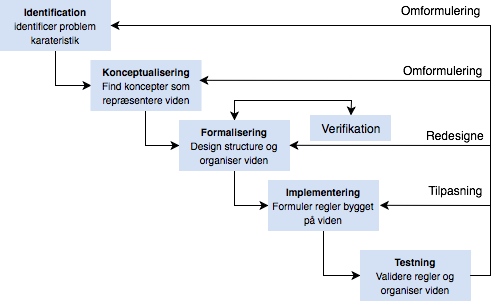
\includegraphics[width=1\textwidth]{Statusseminar/metode.png} 
%%	\caption{XXXX.}
%%	\label{fig:metode}  
%%\end{figure}
%%
%%
%%Da input-output relationen allerede er kendt anvendes supervised machine learning. Da formålet er at identificere hvilken kategori en ny observation tilhører anvendes klassificering.  
%
%%
%%\section{Data forberedelse} / Model
%%- segmentation
%%- farvetransformation - text/tal
%%
%%\section{Klassifikation}
%%\subsection{Machine learning}
%%\subsection{Feature for klassificering}
%%\subsection{Neurale netværk som klassificering}
%%
%%\section{Validering}
%%- klassificering performance matrics 
%%
%%
%%dataindsamling
%%data processering 
%%feature extraction 
%
%
%
%%\vspace{2mm}
%%\begin{longtable}{p{2.5cm}|p{1cm}|p{11cm}}
%%	\caption{**DET HER ER KUN TIL MIG SELV**}
%%	\vspace{2mm}
%%	\label{table:XXX} \\
%%\cellcolor[HTML]{C0C0C0} {\textbf{Data}} & {\cellcolor[HTML]{C0C0C0}\textbf{Antal}} & 
%%{\cellcolor[HTML]{C0C0C0}\textbf{Indhold}} \\ \hline
%%Amgros & 245 & Kontrakt start, ATC-kode, Varenummer 2017, Lægemiddel 2017, Dispenseringsform 2017, Styrke 2017, Pakningsstørrelse 2017, Varenummer 2018, Lægemiddel 2018, Dispenseringsform 2018, Styrke 2018, Pakningsstørrelse 2017, Bemærkning, Rekommenderet.\\ \hline
%%SRN & 5397 & ATC-koder, Matchstatus, Generisk navn, Firma, Varenummer, Forv. Varenummer, SA-Gl.Vnr (Kig Amgros estimering), Varenummerskift – 1 er skift 0 fortsætter (Kig Amgros estimering), Varenavn, Disponeringsform, Styrke, Pakning, Udbudsgruppe, Udbudsnummer (1-730), Vinder (1, 2, 3, 4, 5, 1x, 2x, BA, k), RADS-MR (0, 1) (RADS- medicin rådet måske medicinrådet??), Amg. Est., Budget pakning, Rev. Pakning, Bemærkning, SAIP/Pakning, AIP/Pakning,
%%AIP/Enhed, Enh./Paking , Budget slut, Indkøb start, Indkøb slut, Leadtime, Ingen prisvisning, Modified, ID, Created.\\ \hline
%%Problem & 103 & ATC-kode, Generisk navn, Firma, Varenummer, Varenavn, Udbudsgruppe, Udbudsnummer, Vinder, Debitor, Problemstilling/Bemærkning, Konsekvens, Simpel SAID-sag oprettet, Udfyldt af, Dato. \\ \hline
%%\end{longtable}